%% This file was auto-generated by IPython.
%% Conversion from the original notebook file:
%% stat_hadoop_rand_proj.ipynb
%%
\documentclass[11pt,english,fleqn]{article}

%% This is the automatic preamble used by IPython.  Note that it does *not*
%% include a documentclass declaration, that is added at runtime to the overall
%% document.

\usepackage{amsmath}
\usepackage{amssymb}
\usepackage{graphicx}
\usepackage{ucs}
\usepackage[utf8x]{inputenc}

% needed for markdown enumerations to work
\usepackage{enumerate}

% Slightly bigger margins than the latex defaults
\usepackage{geometry}
\geometry{verbose,tmargin=3cm,bmargin=3cm,lmargin=2.5cm,rmargin=2.5cm}

% Define a few colors for use in code, links and cell shading
\usepackage{color}
\definecolor{orange}{cmyk}{0,0.4,0.8,0.2}
\definecolor{darkorange}{rgb}{.71,0.21,0.01}
\definecolor{darkgreen}{rgb}{.12,.54,.11}
\definecolor{myteal}{rgb}{.26, .44, .56}
\definecolor{gray}{gray}{0.45}
\definecolor{lightgray}{gray}{.95}
\definecolor{mediumgray}{gray}{.8}
\definecolor{inputbackground}{rgb}{.95, .95, .85}
\definecolor{outputbackground}{rgb}{.95, .95, .95}
\definecolor{traceback}{rgb}{1, .95, .95}

% Framed environments for code cells (inputs, outputs, errors, ...).  The
% various uses of \unskip (or not) at the end were fine-tuned by hand, so don't
% randomly change them unless you're sure of the effect it will have.
\usepackage{framed}

% remove extraneous vertical space in boxes
\setlength\fboxsep{0pt}

% codecell is the whole input+output set of blocks that a Code cell can
% generate.

% TODO: unfortunately, it seems that using a framed codecell environment breaks
% the ability of the frames inside of it to be broken across pages.  This
% causes at least the problem of having lots of empty space at the bottom of
% pages as new frames are moved to the next page, and if a single frame is too
% long to fit on a page, will completely stop latex from compiling the
% document.  So unless we figure out a solution to this, we'll have to instead
% leave the codecell env. as empty.  I'm keeping the original codecell
% definition here (a thin vertical bar) for reference, in case we find a
% solution to the page break issue.

%% \newenvironment{codecell}{%
%%     \def\FrameCommand{\color{mediumgray} \vrule width 1pt \hspace{5pt}}%
%%    \MakeFramed{\vspace{-0.5em}}}
%%  {\unskip\endMakeFramed}

% For now, make this a no-op...
\newenvironment{codecell}{}

 \newenvironment{codeinput}{%
   \def\FrameCommand{\colorbox{inputbackground}}%
   \MakeFramed{\advance\hsize-\width \FrameRestore}}
 {\unskip\endMakeFramed}

\newenvironment{codeoutput}{%
   \def\FrameCommand{\colorbox{outputbackground}}%
   \vspace{-1.4em}
   \MakeFramed{\advance\hsize-\width \FrameRestore}}
 {\unskip\medskip\endMakeFramed}

\newenvironment{traceback}{%
   \def\FrameCommand{\colorbox{traceback}}%
   \MakeFramed{\advance\hsize-\width \FrameRestore}}
 {\endMakeFramed}

% Use and configure listings package for nicely formatted code
\usepackage{listingsutf8}
\lstset{
  language=python,
  inputencoding=utf8x,
  extendedchars=\true,
  aboveskip=\smallskipamount,
  belowskip=\smallskipamount,
  xleftmargin=2mm,
  breaklines=true,
  basicstyle=\small \ttfamily,
  showstringspaces=false,
  keywordstyle=\color{blue}\bfseries,
  commentstyle=\color{myteal},
  stringstyle=\color{darkgreen},
  identifierstyle=\color{darkorange},
  columns=fullflexible,  % tighter character kerning, like verb
}

% The hyperref package gives us a pdf with properly built
% internal navigation ('pdf bookmarks' for the table of contents,
% internal cross-reference links, web links for URLs, etc.)
\usepackage{hyperref}
\hypersetup{
  breaklinks=true,  % so long urls are correctly broken across lines
  colorlinks=true,
  urlcolor=blue,
  linkcolor=darkorange,
  citecolor=darkgreen,
  }

% hardcode size of all verbatim environments to be a bit smaller
\makeatletter 
\g@addto@macro\@verbatim\small\topsep=0.5em\partopsep=0pt
\makeatother 

% Prevent overflowing lines due to urls and other hard-to-break entities.
\sloppy

\setlength{\mathindent}{0pt}
\setlength{\parindent}{0pt}
\setlength{\parskip}{8pt}
\begin{document}

\subsubsection{Paralel Rasgele Izdusumu}

Rasgele yansitma teknigi $m \times b$ boyutunda bir matrisi $n \times k$
boyutunda ve her hucresinde $N(0,1)$ dagilimindan gelen bir sayi iceren
matris ile carpmak sonunda elde edilir. Boylece ana veri matrisi
``yansiltilmis'' olur, boyut azaltmak icin cok kullanisli bir tekniktir,
cunku elde edilen matrisin ana matris $A$'nin ``menzilini'' iyi temsil
ettigi ispatlanmistir. Daha fazla detay icin Rasgele Izdusumu ile SVD
yazisina bakabilirsiniz.

Esle/indirge ortaminda rasgele yansitma icin once Matris Carpimi adli
yaziya da bakmak gerekebilir. Bu yazida iki matris arasindaki carpima
``satir bakisi'' bizim icin gerekli. Cunku carpimin solunda $m \times n$
boyutundaki matrisin verileri bize satir satir geliyor, yani her $m$
satirdan sadece bir tanesine bakarak islem yapiyoruz. Faraziyemiz $n$'in
de buyuk olabilmesine ragmen en azindan $n$ tane veri noktasini tek bir
makinada isleyebilecegimiz.

Satir bakisina donersek, bu carpim gorusune gore soldaki her satir icin,
o satirdaki bir ogeyi sagda ona tekabul eden $n \times k$ boyutundaki
matrisin satiriyla (yani her gelen satirin 5. ogesi sagdaki matrisin 5
satirin tamami ile) carpip, sonuc olan ``carpilmis'' satirlari
birbiriyle topluyoruz. Bu Hadoop veri isleme mentalitesine uygun cunku
her seferinde $A$'nin tek bir satirina bakiyoruz.

Sagdaki rasgele sayilar iceren matris kritik. Biz bu matrisi bellekte
tutmamaya karar verdik, cunku $n$ sayisi da buyuk olabilir, her ne kadar
$k$ kucuk olsa da (cogunlukla 100 civari) yine de bu kadar bellegi eger
mumkun ise israf etmemek en iyisi.

\begin{codecell}
\begin{codeinput}
\begin{lstlisting}
imshow(imread("proj.png"))
\end{lstlisting}
\end{codeinput}
\begin{codeoutput}
\begin{verbatim}
<matplotlib.image.AxesImage at 0x42d3a90>
\end{verbatim}
\begin{center}
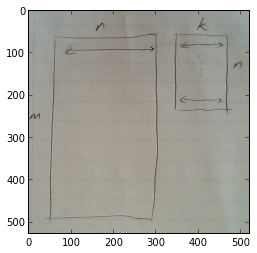
\includegraphics[width=0.7\textwidth]{stat_hadoop_rand_proj_files/stat_hadoop_rand_proj_fig_00.png}
\par
\end{center}
\end{codeoutput}
\end{codecell}
Eger bellekte tutmuyorsak rasgele matrisin degerlerini her seferinde
tekrar uretmek gerekir. Hiz acisindan performans cok kotu olmayacaktir,
cunku rasgele sayi uretimi toplama, carpma, $mod$ gibi direk
matematiksel hesaplar ile yapilir.

Fakat burada onemli bir diger konu sudur: her $A$ satiri icin ayni
rasgele matrisi arka arkaya uretebilmeliyiz.

Bu problemin en basit cozumu rasgele sayi uretimi icin tohum (seed)
kullanimidir. Eger tohum kullanilmazsa, Python random paketindeki
uretici cagrilar gunun zamanina gore bir tohum kullanirlar, ve boylece
her cagri degisik bir sayi uretir. Fakat rasgele sayi uretimini, ``her
seferinde ayni sekilde'' yaptirmanin yolu vardir, bunun icin tohum
disaridan set edilir ve boylece ayni tohumdan baslayan rasgele sayi
uretim zinciri hep ayni olur. Rasgele sayi uretimi deterministik bir
algoritmadir, zaten literaturde bu islem ``yari rasgele sayi uretimi
(pseudorandom number generation)'' olarak gecer.

\begin{codecell}
\begin{codeinput}
\begin{lstlisting}
import random

# tohumsuz, bu kod her seferinde degisik sayi uretir
print random.gauss(0,1), random.gauss(0,1)
print random.gauss(0,1), random.gauss(0,1)

\end{lstlisting}
\end{codeinput}
\begin{codeoutput}
\begin{verbatim}
-0.111385434078 -0.921948609235
1.43737370538 -0.299564009187
\end{verbatim}
\end{codeoutput}
\end{codecell}
\begin{codecell}
\begin{codeinput}
\begin{lstlisting}
# tohumlu

random.seed(100000)
print random.gauss(0,1), random.gauss(0,1)
random.seed(100000)
print random.gauss(0,1), random.gauss(0,1)

\end{lstlisting}
\end{codeinput}
\begin{codeoutput}
\begin{verbatim}
1.46560757321 0.974749135866
1.46560757321 0.974749135866
\end{verbatim}
\end{codeoutput}
\end{codecell}
Ustteki kodda ayni tohumu verince arka arkaya uretilen iki (ya da daha
fazla) ``rasgele'' sayinin hep ayni oldugunu goruyoruz.

Rasgele matrise donersek, eger bu matrisin her veri satiri icin hucre
degerlerinin ayni sekilde uretilmesini istiyorsak, tohum kullanmaliyiz.
Tohum degeri ne olacak? Bu deger mesela $n \times k$ boyutundaki rasgele
matris icin indis degerleri yanyana koyularak uretilebilir, mesela 111.
satir ve 2. kolon icin 1112 tohum degeri kullanilir, ve bu tohumla tek
bir rasgele sayi uretilir, (111,2) hucresine konulur ve sonraki indis
icin yeni bir tohum kullanilir.

Ust uste cakismalar olabilir tabii ki, mesela 11. satir 12. kolon da
ustteki tohumla ayni sonucu getirir, ama bu tur nadir cakismalar o kadar
onemli degil, sonucta rasgele sayilarla ugrasiyoruz, ``yeterince
raslantisal olmalari'' kafi.

Altta bu veri matrisini satir satir carpip yansitilmis yeni bir matrisi
ureten mrjob programini bulabilirsiniz.

\begin{codecell}
\begin{codeinput}
\begin{lstlisting}
print(open("mrproj.py").read())
\end{lstlisting}
\end{codeinput}
\begin{codeoutput}
\begin{verbatim}
from mrjob.job import MRJob
from mrjob.protocol import PickleProtocol, RawValueProtocol
import numpy as np, sys
import random

class MRProj(MRJob):
    INTERNAL_PROTOCOL = PickleProtocol
    OUTPUT_PROTOCOL = RawValueProtocol
    
    def __init__(self, *args, **kwargs):
        super(MRProj, self).__init__(*args, **kwargs)
        self.k = 3
        
    def mapper(self, key, line):
        line_vals = map(np.float,line.split())
        result = np.zeros(self.k)
        for j,val in enumerate(line_vals):
            for i in range(self.k):
                random.seed(int(j + i))
                result[i] += val*random.gauss(0,1)
        yield (None,",".join(map(str,result)))
            
if __name__ == '__main__':
    MRProj.run()
\end{verbatim}
\end{codeoutput}
\end{codecell}
Tek bir esle cagrisi var, cunku carpim islemi oldukca basit, indirgeme
islemine gerek yok.

Satirlar icin anahtar kullanmiyoruz, yani verinin paralel islenirken
nasil yuk dagitimi yapildigina gore sonuc matrisinin sirasi ana matrisin
satir sirasina uymayabilir. Fakat satir sirasi bizim icin cogunlukla
onemli olmuyor (kolon sirasi onemli), her satir digerinden ayri bir
verini temsil eder cogunlukla. Eger zamansal bir boyut var ise, o bilgi
ayri bir kolon (mesela tarih, zaman damgasi -timestamp-) olarak veride
bulunurdu.

\begin{codecell}
\begin{codeinput}
\begin{lstlisting}
!python mrproj.py A_matrix > /tmp/out
\end{lstlisting}
\end{codeinput}
\begin{codeoutput}
\begin{verbatim}
using configs in /home/burak/.mrjob.conf
creating tmp directory /tmp/mrproj.burak.20131002.173222.276299
\end{verbatim}
\begin{verbatim}
writing to /tmp/mrproj.burak.20131002.173222.276299/step-0-mapper_part-00000
Counters from step 1:
  (no counters found)
Moving /tmp/mrproj.burak.20131002.173222.276299/step-0-mapper_part-00000 -> /tmp/mrproj.burak.20131002.173222.276299/output/part-00000
Streaming final output from /tmp/mrproj.burak.20131002.173222.276299/output
removing tmp directory /tmp/mrproj.burak.20131002.173222.276299
\end{verbatim}
\end{codeoutput}
\end{codecell}
\begin{codecell}
\begin{codeinput}
\begin{lstlisting}
!head -10 /tmp/out
\end{lstlisting}
\end{codeinput}
\begin{codeoutput}
\begin{verbatim}
20.2369671373,13.9358970644,0.524561578258
19.8581349841,13.7724732852,5.23992858318
27.6790861925,18.8833585029,-1.56199395804
9.3255498646,7.52383094482,2.58977793605
27.3677257439,33.0438553532,18.4819155509
27.6790861925,18.8833585029,-1.56199395804
9.3255498646,7.52383094482,2.58977793605
27.3677257439,33.0438553532,18.4819155509
27.6790861925,18.8833585029,-1.56199395804
9.3255498646,7.52383094482,2.58977793605
\end{verbatim}
\end{codeoutput}
\end{codecell}
Performans Iyilestirmeleri

Ustteki kod daha hizli olabilir. Diyelim ki $n$'in milyonlarda oldugu
sartlari da hizli bir sekilde isleyebilmek istiyoruz. Fakat bu noktada
kendimize su soruyu sormamiz gerekir: hangi sartlarda $n$ milyonlari
bulacaktir?

Buyuk bir ihtimalle bu durum eger bolca kategorik veri boyutu var ise
ortaya cikar. Kategorik verileri bildigimiz gibi 1-in-n, ya da one-hot
kodlama (encoding) ile temsil ediyoruz, bu demektir ki 1000 tane farkli
deger icerebilen tek bir kolon, 1000 tane yeni kolon haline geliyor.
Bazi boyutlarin (mesela web sayfa ismi, URL degeri) tasiyan veri
setlerinde tekil (unique) degerlerin milyonlar hatta milyara
varabilecegini dusunursek asiri yuksek $n$ rakamlarinin nereden
geldigini anlariz.

Ama bunun bize ek bir faydasi var: 1-in-n kodlamasi var ise, bu her
satirda cok fazla sifir olacak demektir, ve icinde cok sifiri olan
vektorleri / matrisleri seyrek matrisler ile cok rahat sekilde temsil
edebiliriz.

\begin{codecell}
\begin{codeinput}
\begin{lstlisting}
print(open("mrprojs.py").read())
\end{lstlisting}
\end{codeinput}
\begin{codeoutput}
\begin{verbatim}
from mrjob.job import MRJob
from mrjob.protocol import PickleProtocol, RawValueProtocol
import numpy as np, sys, itertools
from scipy import sparse
import random

class MRProj(MRJob):
    INTERNAL_PROTOCOL = PickleProtocol
    OUTPUT_PROTOCOL = RawValueProtocol
    
    def __init__(self, *args, **kwargs):
        super(MRProj, self).__init__(*args, **kwargs)
        self.k = 3
        
    def mapper(self, key, line):
        line_vals = map(np.float,line.split())
        line_sps = sparse.coo_matrix(line_vals,shape=(1,len(line_vals)))
        result = np.zeros(self.k)
        for xx,j,v in itertools.izip(line_sps.row, line_sps.col, line_sps.data):
            for i in range(self.k):
                random.seed(int(j + i))
                result[i] += v*random.gauss(0,1)
        yield (None,",".join(map(str,result)))
            
if __name__ == '__main__':
    MRProj.run()
\end{verbatim}
\end{codeoutput}
\end{codecell}
Ustteki kodda her satiri okur okumaz hemen onu bir seyrek matrise
ceviriyoruz. Simdi en kritik numara: itertools.izip cagrisi ile bu
seyrek matrisin sadece sifir olmayan degerlerini ziyaret ediyoruz. Eger
1000 tane kolon var ise, ama bu 1000 kolonun 20 tanesi dolu ise, bu 50
kat bir performans iyilestirmesi saglayacak demektir (bu arada seyrek
verilerde yuzde 2 doluluk gayet normal bir rakamdir). Sadece dolu
hucreleri ziyaret ediyoruz, ayrica izip bu dolu hucrelerin indis
degerlerini de bize geri getiriyor, biz de bu degerleri seed icin
onceden oldugu gibi kullaniyoruz.

Sonuclara bakalim:

\begin{codecell}
\begin{codeinput}
\begin{lstlisting}
!python mrprojs.py A_matrix > /tmp/out
!head -10 /tmp/out

\end{lstlisting}
\end{codeinput}
\begin{codeoutput}
\begin{verbatim}
using configs in /home/burak/.mrjob.conf
creating tmp directory /tmp/mrprojs.burak.20131002.173847.485554
writing to /tmp/mrprojs.burak.20131002.173847.485554/step-0-mapper_part-00000
\end{verbatim}
\begin{verbatim}
Counters from step 1:
  (no counters found)
Moving /tmp/mrprojs.burak.20131002.173847.485554/step-0-mapper_part-00000 -> /tmp/mrprojs.burak.20131002.173847.485554/output/part-00000
Streaming final output from /tmp/mrprojs.burak.20131002.173847.485554/output
removing tmp directory /tmp/mrprojs.burak.20131002.173847.485554
\end{verbatim}
\begin{verbatim}
20.2369671373,13.9358970644,0.524561578258
19.8581349841,13.7724732852,5.23992858318
27.6790861925,18.8833585029,-1.56199395804
9.3255498646,7.52383094482,2.58977793605
27.3677257439,33.0438553532,18.4819155509
27.6790861925,18.8833585029,-1.56199395804
9.3255498646,7.52383094482,2.58977793605
27.3677257439,33.0438553532,18.4819155509
27.6790861925,18.8833585029,-1.56199395804
9.3255498646,7.52383094482,2.58977793605
\end{verbatim}
\end{codeoutput}
\end{codecell}
Daha onceki sonuclar ile ayni (rasgelelik var ama seed degerleri
degismedi, o sebeple ayni sonucu aldik, bu iyi).

Bir kontrol daha var, eger rasgelelik bazli yansitma iyi yapildiysa, $A$
matrisini izdusumunu aldiktan daha once anlattigimiz teknik ile SVD
hesabini cok rahat bir sekilde yapabilmeliyiz. Bunun icin izdusumunu
/tmp/Y icine yazacagiz, ve ardindan daha onceki QR bazli teknikle SVD
hesabini yapacagiz. Ardindan pur SVD ile $A$'yi isleyecegiz ve sonuc $U$
matrisindeki en buyuk iki tekilsel (singular) degeri her iki teknikten
alip ekranda grafikleyecegiz.

\begin{codecell}
\begin{codeinput}
\begin{lstlisting}
!python mrprojs.py A_matrix > /tmp/Y

import numpy as np
import numpy.linalg as lin
import matplotlib.pyplot as plt

n = 4; k = 3
A = np.loadtxt('A_matrix')
Y = np.loadtxt("/tmp/Y",delimiter=',')

Q, xx = lin.qr(Y)
B = np.dot(Q.T,A)
Uhat, Sigma, V = lin.svd(B)
U = np.dot(Q, Uhat)

plt.plot(U[:,0],U[:,1],'r+')
plt.hold(True)

U, Sigma, V = lin.svd(A);
plt.plot(U[:,0],U[:,1],'bx')

plt.show()

\end{lstlisting}
\end{codeinput}
\begin{codeoutput}
\begin{verbatim}
using configs in /home/burak/.mrjob.conf
creating tmp directory /tmp/mrprojs.burak.20131002.185301.111949
writing to /tmp/mrprojs.burak.20131002.185301.111949/step-0-mapper_part-00000
\end{verbatim}
\begin{verbatim}
Counters from step 1:
  (no counters found)
Moving /tmp/mrprojs.burak.20131002.185301.111949/step-0-mapper_part-00000 -> /tmp/mrprojs.burak.20131002.185301.111949/output/part-00000
Streaming final output from /tmp/mrprojs.burak.20131002.185301.111949/output
removing tmp directory /tmp/mrprojs.burak.20131002.185301.111949
\end{verbatim}
\begin{center}
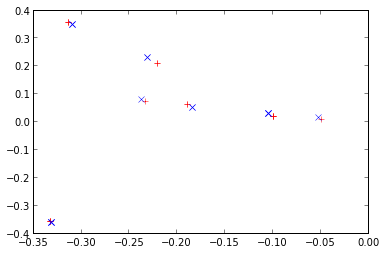
\includegraphics[width=0.7\textwidth]{stat_hadoop_rand_proj_files/stat_hadoop_rand_proj_fig_01.png}
\par
\end{center}
\end{codeoutput}
\end{codecell}
Sonuclar mukemmel.

\end{document}
